\section{Lua-parserns implementation}

Implementationen är indelad i fyra komponenter. När parsern startas börjar
en syntaktisk analysator parsa input från rot-noden.  Det första som görs är
ett anrop till den andra komponenten, lexern. Lexern läser input tecken för
tecken och tokeniserar värden som sedan returneras till den syntaktiska
analysatorn var den används för att välja produktionsregel. Utanför lexern
hanteras inte enskilda tecken utan enbart tokens.  Utöver dessa två
komponenter finns en separat uttrycksparser samt ett delegerare som producerar
ett syntaxträd vilket slutligen returneras till programmet som anropat parsern
i första hand.

\subsection{Lexer}

Lexern läser input enligt en reguljär grammatik och gör detta som en
deterministisk ändlig automat. När parsningen av en token börjar hämtas det
aktuella tecknet i input strängen och lexern går sedan genom en serie villkor
för att bestämma var en token slutar och av vilken typ den är. När en token
slutat har automaten nått sitt slutliga tillstånd och tokenvärdet returneras.
Slutligen återgår automaten till utgångsläget för att vänta på nästa
förfrågan.

Tokentyperna som lexern användar är: \textit{``End-of-file''} (EOF),
teckensträngs-litteral, nyckelord, identifierare, tal-litteral, symbol,
boolean samt nil. Dessa definieras som uppräkningsflaggor (enum flag) för att
kunna jämföras med bit operationer. När en token identifieras av lexern
returneras den som ett objekt med attribut för tokentypen, dess index-position
i input-teckensträngen, dess rad och kolumn i input samt dess tokenvärde.

\subsubsection{Blanksteg och kommentarer}

Eftersom blanksteg utgör 40\% av implementationens kod kan det konstateras att
lexern spenderar en väsentlig del av sin tid på blanksteg. Det första lexern
gör när den anropas är att anropa en funktion som ignorerar alla
blankstegstecken som hittas.

Eftersom token-objekt innehåller information om rad och kolumn i input
memoreras varje radförändringen i funktionen som ignorerar blanksteg.
Ytterligare lagras input-positionen när en rad påbörjas. När ett tokenobjekt
skapas subtraheras radens startposition från den nuvarande input-positionen
och bildar därmed kolumnen.

Kompilatorer kan ignorera kommentarer eftersom de inte innehåller semantiska
värden men eftersom målet med denna implementation är användningen för
kodanalys sparas även kommentarer. Detta görs genom att söka efter
avgränsarsymbolen (\verb+--+) och lagra dess information i en separat tabell
som slutligen anknyts till det returnerade syntaxträdet.

\subsubsection{Identifierare och nyckelord}

Från och med Lua 5.2 kan variabelnamn, eller s.k. identifierare, endast bestå av
bokstäver, siffror och understreck i ASCII-uppsättningen. Ytterligare kan ett
variabelnamn inte börja med en siffra \citep{luaref}.

Nyckelord är terminaler med samma regler som identifierare och därmed kan de
använda samma logik för att avskilja giltiga tecken. En skillnad mellan
parser-implementationen och Lua-grammatiken är åtskiljandet mellan nyckelord
och datatyperna nil, boolean.

Med att granska grammatiken för tokentyperna kan det utläsas att enbart nil,
boolean, nyckelord samt identifierare kan börja med en bokstav. Eftersom
lexern arbetar tecken för tecken kan detta användas som en villkorsförgrening.
Om en ny token börjar med en bokstav måste det tillhöra någon av dessa fyra
tokentyper, ytterligare vet vi att tokentypen slutar där ett tecken inte är en
bokstav, en siffra eller ett understreck.

Implementationen av denna fögrerning görs genom att läsa ASCII-koden för
tecknet och granska om det är en bokstav eller ett understreck. Om testet
lyckas fortsätter lexern att acceptera tecken så länge som teckenkoden tillhör
serien för bokstäver, siffror och understreck. När testet misslyckas betyder
det att denna token tagit slut och nu kan lexern granska om värdet är lika med
ett boolean-värde, ett nil-värde, ett av nyckelorden eller inte tillhör någon
av dessa och därmed är en identifierare.

\subsubsection{Symboler}

Identifieringen av symboler implementeras med en serie switch- och
if-satser vilka granskar vilka tecken framåt i input tillhör en giltig
symbol. När den längsta möjliga symbolen identifieras returneras den.

Luas giltiga symboler är:
\begin{verbatim}
. .. ... : :: ; # = == > >= < <= ~= { } ( ) [ ] ^ % * / - +
\end{verbatim}

\subsubsection{Litteraler}

Lua stöder tal likt vanliga programmeringsspråk men har även stöd för
hexadecimaltal innehållande en valfri binär expontent. Implementationen läser
input och verifierar att talet är giltigt. När token-värdet identifierats
konverteras det till ett flyttal och returneras.

Teckensträngar i Lua börjar antingen med enkla citationstecken (\verb+'+)
eller dubbla citationstecken (\verb+"+) och samma avgränsarsymbol förväntas
innan raden tar slut. Lua tillåter dock att man inaktiverar en symbol såsom
citations- eller radbrytningstecken genom att använda ett omvänt snedstreck
(\verb+\+). En annan användning för det omvända snedstrecket är att definiera
en styrkodsekvens.  När lexern hittar ett snedstreck inom en
teckensträngslitteral granskas först giltiga styrkodssekvenser och om ingen
identifieras inaktiveras följande tecken i input.

\subsection{Syntaktisk analysator}

Den syntaktiska analysatorn är implementerad som en rekursivt nedstigande
parser för en LL(1)-grammatik. Parsern börjar från
rot-noden. Denna nod består av en block-nod med en obestämd mängd
satser-noder. Varje nodtyp, eller regel, är implementerad som en funktion som
rekursivt anropar andra regelfunktioner och slutligen returnerar ett
syntaxträd över sin struktur. När input strängen tagit slut har det
slutgiltiga syntaxträdet returnerats till rot-noden och kan därefter förmedlas
till programmet som begärt informationen.

Mycket av den syntaktiska analysatorns grammatik är samma som den ursprungliga
Lua-grammatiken. Dock har vissa finjusteringar gjorts för att bland annat
kunna åtskilja variabeldeklarationer från funktionsanrop.

% Dessa två sats-typer
% skulle normalt kräva fler \textit{``lookahead''} tokens för att kunna
% identifieras korrekt. Implementationen har istället implementerat
% funktionalitet för memoisation. Detta innebär att det första alternativet
% testas och om det misslyckas används istället det andra alternativet.

\subsubsection{Hjälp-funktioner}

För att underlätta hanteringen av produktionsregler samt kommunikationen med
lexer-komponenten används vissa hjälp-funktioner.

Kommunikationen med lexern sker med en \textit{next()}-funktion. Funktionen
ansvarar även för att parsern skall ha tillgång till en
\textit{``lookahead''}-token som krävs för att syntaxen skall kunna
analyseras. När funktionen anropas ersätts den aktuella token med
\textit{``lookahead''}-token.  Efter detta anropas lexern och dess resultat
sparas som \textit{``lookahead''}-token. Dessa tokens lagras som variabler tillgängliga för
hela implementationen.

Ytterligare existerar två viktiga hjälp-funktioner för att hålla
implementationen mer läslig. \textit{expect()}-funktionen anropas med ett
tokenvärde, som jämförs med den aktuella token. Stämmer bägge överens hämtas
nästa token mha. \textit{next()} metoden. Om de inte överenstämmer skapas ett
felmeddelande eftersom syntaxen inte är korrekt. Denna funktion används för
att granska terminaler när en produktionsregel hittats.

Den andra väsentliga hjälp-funktionen är \textit{consume()} som likt
\textit{expect()} granskar om ett tokenvärde överenstämmer med den aktuella
token. Skillnaden är att \textit{consume()} inte skapar ett felmeddelande utan
returnerar istället sant eller falskt. Detta används för att granska valfria
delar av en produktionsregel, t.ex. if-satser som har en valfri \textit{else}
komponent.

\subsubsection{EBNF-notation till JavaScript-kod}

Processen att omvandla EBNF-notation är en enkel process när eliminieringen av
$\epsilon$ gjorts. Alternering implementeras som switch-satser, villkor som
if-satser och repetition som while-, for- eller do-satser.

För att minimera komplexiteten av parsern har implementationen delat upp
produktionsregeln \bnfrule{sats} så att den enbart identifierar vilken typ av
sats det handlar om utgående från den första terminalen. Efter att satsen
identifieras anropas funktionen knyten till satstypen.

Ytterligare optimerar jag sats-grammatiken med att ordna reglerna enligt
populariteten baserad på en provtagning av ett exempelprogram (bilaga 2).

Den nya \bnfrule{sats}-grammatiken visas i figur~\ref{fig:stat}.

\begin{figure}[ht]
  \setlength{\grammarindent}{5em}
  \begin{grammar}
    \singlespace\small%
    \fontfamily{lmr}\selectfont
    <sats> ::= "local" <local-sats>
      \alt "if" <if-sats>
      \alt "return" <retur-sats>
      \alt "function" <funktion-sats>
      \alt "while" <while-sats>
      \alt "for" <for-sats>
      \alt "repeat" <repeat-sats>
      \alt "break" <break-sats>
      \alt "do" <do-sats>
      \alt "goto" <goto-sats>
      \alt "::" <label-sats>
      \alt ";"
      \alt <deklaration-eller-anrop-sats>
  \end{grammar}
  \caption{Parser-implementationens produktionsregel för en sats}
  \label{fig:stat}
\end{figure}

\subsubsection{Implementation av produktionsregler}

Som exempel omvandlas följande if- samt while-sats till
JavaScript-motsvarigheterna i figur~\ref{fig:ifstat}.

\begin{figure}[ht]
  \setlength{\grammarindent}{3em}
  \begin{grammar}
    \singlespace\small%
    \fontfamily{lmr}\selectfont
      <sats> ::= "if" <if-sats> | "while" <while-sats> | \ldots

      <if-sats> ::= "if" <uttryck> "then" <block> \{"elseif" <uttryck> "then" <block>\}
      ["else" <block>] "end"

      <while-sats> ::= "while" <uttryck> "do" <block> "end"
  \end{grammar}
  \begin{minipage}[t]{0.5\textwidth}
  \lstinputlisting[title="",language=Javascript]%
    {figures/tex/if-statement.js}
  \end{minipage}
  \begin{minipage}[t]{0.5\textwidth}
  \lstinputlisting[title="",language=Javascript]%
    {figures/tex/while-statement.js}
  \end{minipage}
  \caption{Produktionsregelerna för if- och while-satser i JavaScript-kod}
  \label{fig:ifstat}
\end{figure}

\subsection{Uttrycksparser}

Lua-grammatikens uttrycksregel, \bnfrule{expr}, utnyttjar vänsterrekursion,
vilket inte är möjligt i rekursivt nedstigande parsers eftersom de hamnar i en
oändlig upprepning.

Uttrycksregeln består av en serie andra icke-terminaler vilkas funktioner är
svåra att få ett grepp om och därför kommer vi att expandera och analysera
alla delregler för att slutligen få en fungerande och förhoppningsvis mer
organiserad produktionsregel för uttryck.

Processen för att införa detta kommer bestå av tre steg, där det det första
steget visar den ursprungliga regeln, det andra steget visar resultatet från
att eliminera vänsterrekursion och det tredje steget visar regeln skriven utan epsilon.
Med att omforma regeln till att använda repetition istället för epsilon är
regeln färdig för att översättas till kod.

\subsubsection{Gruppering av uttryck}

För att lättare arbeta med definitioner indelas uttryck i binära och unära
operationer, prefix uttryck samt primära uttryck. Primära uttryck består av de
kvarstående alternativen, huvudsakligen datatyper.

\begin{description}
  \setlength{\grammarindent}{5em}
  \item[Ursprungsregel] \hfill
    \begin{grammar}
      \singlespace\small%
      \fontfamily{lmr}\selectfont
      <exp> ::= <primaryexp> | <prefixexp> | <exp> <binop> <exp> | <unop> <exp>

      <primaryexp> ::= \ldots

      <prefixexp> ::= \ldots
    \end{grammar}

  \item[Eliminering av vänsterrekursion] \hfill
    \begin{grammar}
      \singlespace\small%
      \fontfamily{lmr}\selectfont
      <exp> ::= <primaryexp> <exp'> | <prefixexp> <exp'> | <unop> <exp>

      <exp'> ::= <binop> <exp> | $\epsilon$
    \end{grammar}

  \item[Resultat] \hfill
    \begin{grammar}
      \singlespace\small%
      \fontfamily{lmr}\selectfont
      <exp> ::= ( <unop> <exp> | <primaryexp> | <prefixexp> ) \{ <binop> <exp> \}
    \end{grammar}
\end{description}

\subsubsection{Analys av prefixuttryck}

\begin{description}
  \setlength{\grammarindent}{8em}
  \item[Ursprungsregel] \hfill
    \begin{grammar}
      \singlespace\small%
      \fontfamily{lmr}\selectfont
      <prefixexp> ::= <var> | <functioncall> | "(" <exp> ")"

      <var> ::= Name | <prefixexp> "[" <exp> "]" | <prefixexp> "." Name

      <functoincall> ::= <prefixexp> <args> | <prefixexp> ":" Name <args>

      <args> ::= "(" [ <explist> ] ")" | <tableconstructor> | String
    \end{grammar}

    Den fullständiga regeln för \bnfrule{args} finns i bilaga 1, men för
    att hålla grammatiken enkel utelämnas dess helhet här och vi konstaterar
    endast att regeln inte behöver bearbetas mer. Vi expanderar de övriga
    delreglerna för att få en bättre överblick.

    \begin{grammar}
      \singlespace\small%
      \fontfamily{lmr}\selectfont
      <prefixexp> ::= Name | <prefixexp> "[" <exp> "]" | <prefixexp> "." Name
        \alt <prefixexp> <args> | <prefixexp> ":" Name <args>
        \alt "(" <exp> ")"
    \end{grammar}

  \item[Eliminering av vänsterrekursion] \hfill
    \begin{grammar}
      \singlespace\small%
      \fontfamily{lmr}\selectfont
      <prefixexp> ::= Name <prefixexp'> | "(" <exp> ")" <prefixexp'>

      <prefixexp'> ::= "[" <exp> "]" | "." Name <args> | ":" Name <args> |
      $\epsilon$
    \end{grammar}

  \item[Resultat] \hfill
    \begin{grammar}
      \singlespace\small%
      \fontfamily{lmr}\selectfont
      <prefixexp> ::= ( Name | "(" <exp> ")" ) \{ "[" exp "]" | "." Name |
          ":" Name <args> | <args> \}
    \end{grammar}
\end{description}

\subsubsection{Sammanknytning}

Med hjälp av dessa modifieringar har vi nu en produktionsregel för uttryck som
inte använder sig av vänsterrekursion och kan därmed användas i en rekursivt
nedstigande parser.

\setlength{\grammarindent}{6em}
\begin{grammar}
  \singlespace\small%
  \fontfamily{lmr}\selectfont
  <exp> ::= ( <unop> <exp> | <primary> | <prefixexp> ) \{ <binop> <exp> \}

  <primary> ::= "nil" | "false" | "true" | Number | String | "..." |
      <functiondef> | <tableconstructor>

  <prefixexp> ::= ( Name | "(" <exp> ")" ) \{ "[" exp "]" | "." Name |
      ":" Name <args> | <args> \}
\end{grammar}

\subsubsection{Operationsprioritet}

Operationsprioritet innebär den logik som bestämmer att multiplikation
prioriteras högre än addition och därmed grupperar uttryck såsom \textit{5 + 5
* 2} till \textit{5 + (5 * 2)} istället för \textit{(5 + 5) * 2}. Lua-manualen
nämner att grammatiken inte beskriver operationsprioritet \citep{luaref} men
en lista av på prioriteterna kan hittas i källkoden av Luas egna parser
\citep{lparse} samt i tabell~\ref{tab:precedence}.

\begin{table}[ht]
  \caption{Tabell över Luas operatorprioritet}
  \begin{tabular}{l l}
    Operator & Prioritet \\
    \hline
    \verb|^| & 10 \\
    \verb|* / %| & 7 \\
    \verb|+ -| & 6 \\
    \verb|..| & 5 \\
    \verb|== < <= > >= ~=| & 3 \\
    \verb|and| & 2 \\
    \verb|or| & 1
  \end{tabular}
  \label{tab:precedence}
\end{table}

En implementationsmöjlighet som Lua själv använder är att spjälka ut
funktion som parsar uttryck till en ny funktionen som tar emot
operatorprioriteten som ett argument med den lägsta prioriteten som
ursprungsläge. Funktionen spjälker sedan uttrycket i ett vänsterled, ett
högerled och operatorn mellan dessa. Om operatorns prioritet är högre än
prioriteten som givits som argument parsar funktionen rekursivt operationens
högerled och skapar en ny operationsgruppering så länge som prioriteten är
högre. Om operatorns prioritet är lägre än eller samma som argumentets
prioritet kommer iterationen att avbrytas och det nuvarande uttrycket att
returneras till det högra ledet. Eftersom ursprungslägets prioritet är den
lägsta kommer alltid ett uttryck att fortsätta så länge som en operator kan
hittas.

Denna algoritm kallas för \textit{``operator precedence''} parsning och
använder sig av \textit{``nerifrån-och-upp''}-strategin. Pseudokoden för en
implementation visas i figur~\ref{fig:binprecedence} och ett
grupperingsexempel visas i figur~\ref{fig:expressiontree}.

\begin{figure}[ht]
  \lstinputlisting[title="",language=Javascript]%
    {figures/tex/binary-precedence.js}
  \caption{En ``operator precedence''-uttrycksparser.}
  \label{fig:binprecedence}
\end{figure}

\paragraph{Ett steg för steg exempel av parsningen för uttrycket 1 + 2 - 3 * 4
+ 5.}
\hfill

Punkterna 1 till 9 beskriver stegen för det ursprungliga funktionsanropet medan
en underlista representerar stegen i ett rekursivt funktionsanrop.

\begin{enumerate}\itemsep1pt \parskip0pt \parsep0pt
  \item Vänstra ledet har värdet 1 och operatorn är + med en prioritet på 1.
  \item Eftersom prioriteten är högre än ursprungsläget anropar funktionen sig
    själv med den nya prioriteten.
    \begin{enumerate}
      \item Vänstra ledet är 2 och operatorn är - med en prioritet på 1.
      \item Eftersom prioriteten är samma som föregående returneras värdet 2.
    \end{enumerate}
  \item Högra ledet är 2.
  \item En gruppering sker och vänstra ledet blir nu (1 + 2).
  \item Följande operator är - med en prioritet på 1 som är mer än 0 och
    därmed anropar funktionen sig själv.
    \begin{enumerate}
      \item Vänstra ledet är 3 och operatorn är * med en prioritet på 2.
      \item Eftersom 2 är högre än 1 anropar funktionen sig själv.
      \begin{enumerate}
        \item Vänstra ledet är 4 och operatorn är + med en prioritet på 1.
        \item Eftersom 1 är lägre 2 returneras värdet 4.
      \end{enumerate}
      \item Högra ledet är nu 4.
      \item En gruppering sker och vänstra ledet blir nu (3 * 4).
      \item Operatorn är + med en prioritet på 1 vilket är samma som
        argumentets prioritet och därmed returnerar funktionen värdet (3 * 4).
    \end{enumerate}
  \item Högra ledet är nu (3 * 4) och en gruppering sker så att vänstra ledet
    blir ((1 + 2) - (3 * 4)).
  \item Följande operator är + med en prioritet på 1 som är mer än 0 och
    därmed anropar funktionen sig själv.
    \begin{enumerate}
      \item Vänstra ledet är 5 och eftersom ingen operator hittas returneras
        värdet.
    \end{enumerate}
  \item Högra ledet är nu 5 och grupperingen blir (((1 + 2) - (3 * 4)) + (5)).
  \item Eftersom ingen operator kan hittas returneras det slutgiltiga
    uttrycket.
\end{enumerate}

\begin{figure}[ht]
  \includegraphics[width=5cm]{figures/output/expression-tree.pdf}
  \caption{Grupperingsträd av det matematiska uttrycket 1 + 2 - 3 * 4 + 5.}
  \label{fig:expressiontree}
\end{figure}

\subsubsection{Operatorassociativitet}

Operatorassociativitet används för att gruppera operatorer med samma prioritet
och utan användningen av parenteser. De vanliga matematiska operatorerna har ingen
associativitet eftersom $(1 * 2) * 3$ har samma resultat som $1 * (2 * 3)$. I
uttrycksparsern från figur~\ref{fig:binprecedence} hanteras dessa operatorer
som vänsterassociativa och grupperas därmed som $(1 * 2) * 3)$. Detta kan
implementeras godtyckligt.

Lua har dock två operatorer med högerassociativitet, nämligen operatorn för
sammanfogningen av teckensträngar (\textit{..}) samt potensoperatorn
(\textit{\^{}}). Om uttrycket \textit{5\^{}4\^{}3\^{}2} grupperas från vänster likt
addition skulle det se ut som \textit{((5\^{}4)\^{}3)\^{}2}, vilket inte har
samma resultat som det korrekta högerassociativa \textit{5\^{}(4\^{}(3\^{}(2)))}.

Implementationen för detta hittas i figur~\ref{fig:rightassociative} och är en
modifiering av algoritmen i figur~\ref{fig:binprecedence}. Lösningen utgörs av
att subtrahera 1 från operatorprioriteten om en högerassociativ regel hittas
innan det högra ledet parsas. Detta orsakar en omvändning i grupperingen.

\begin{figure}[ht]
  \lstinputlisting[title="",language=Javascript]%
    {figures/tex/right-associative.js}
  \caption{Implementation för högerassociativa operatorer.}
  \label{fig:rightassociative}
\end{figure}

\subsubsection{Resultat}

Resultatet av denna omvandling visar sig vara en nära exakt kopia av Luas egna
uttrycksparser med vissa skillnader för operatorassociativitet. Det kan
konstateras att skaparna använt sig av metoden för eliminering av
vänsterrekursion för att omvandla sin tidigare Yacc-skapade parser till en
handskriven rekursivt nedstigande parser.

\subsection{Abstrakt syntaxträd}

Eftersom implementationens mål är att användas som kodanalysator representeras
parsningens syntaxträd som ett abstrakt syntaxträd. Varje nod i trädet
innehåller ett obligatoriskt typ-attribut samt en serie andra attribut som är
nod-specifika. Dessa noder är implementerade som objekt-litteraler och
returneras till det anropande programmet började från programmets rot, Luas
s.k. \textit{``chunk''}.

Implementationen av det abstrakta syntaxträdet är uppbyggt med att varje nod
existerar som en funktion vars ansvar är att skapa en representation av
informationen. Under den syntaktiska analysen delegeras skapandet av noder
till dessa funktioner. För att det anropande programmet skall ha möjlighet att
så enkelt som möjligt omstrukturera syntaxträdet tillgängliggörs dessa
funktioner via parserns API.

Eftersom syntaxträdet representerar en mycket låg nivå i Luas egna parser har
jag valt att ta inspiration av Mozillas Parser API \citep{parserapi}.

Ett exempel på syntaxträd genererat från en parsning visas i
figur~\ref{fig:tool}.

\begin{figure}[ht]
  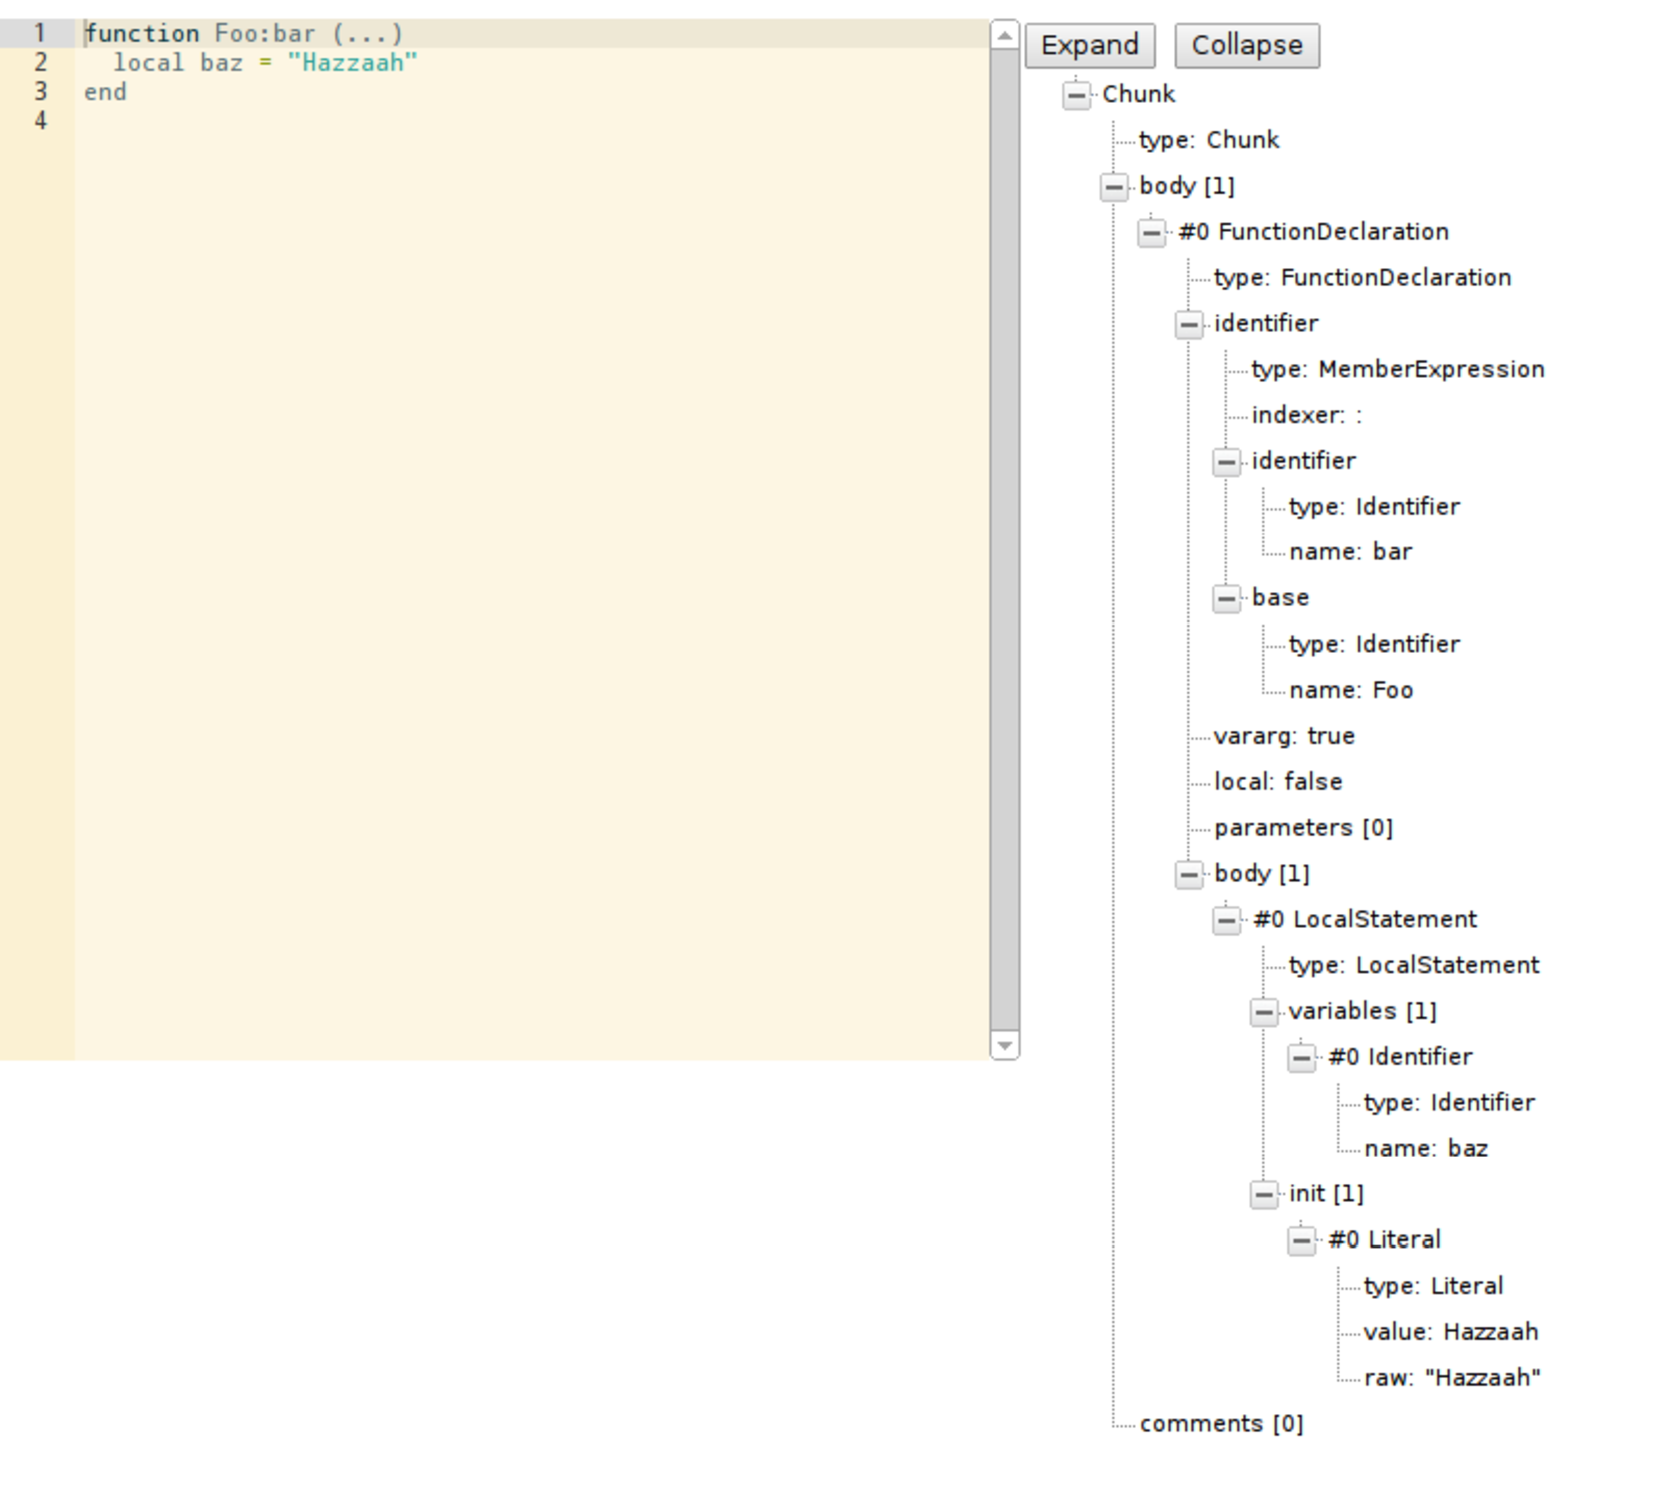
\includegraphics[width=\textwidth]{figures/pdf/tool.pdf}
  \caption{Abstrakt syntaxträd (höger) för parsningen av en Lua-funktion
  (vänster).}
  \label{fig:tool}
\end{figure}

% vim: set tw=78:ts=2:sw=2:et:fdm=marker:wrap:wm=78:ft=tex
% vim: spell spelllang=sv
